\documentclass[11pt]{article}
\usepackage[letterpaper,margin=1in]{geometry}
\usepackage{amsmath,amssymb,booktabs,graphicx,hyperref}
\usepackage[T1]{fontenc}
\hypersetup{colorlinks=true,linkcolor=blue,citecolor=blue,urlcolor=blue}
\title{Feedback Is All You Need}
\author{Research working draft: version 3}
\date{25 October 2026 (UTC)}
\begin{document}
\maketitle
\begin{abstract}
Can a small controller acquire high capability by repeatedly incorporating
feedback? We test a restricted form of this hypothesis rather than assume
that model capacity becomes irrelevant. Across 20 task seeds, four model
sizes, and seven feedback conditions in each of two changing classification
environments, a 161-parameter learner with accurate feedback outperforms a
2,561-parameter frozen learner by 52.91 percentage points on linear rules and
37.32 points on XOR rules. However, when both receive accurate feedback, the
larger model exceeds the smaller by 10.93 points on XOR. A linear model remains
near chance on XOR despite repeated correction. Corruption, latency, and replay
further condition adaptation. These controlled results support feedback as a
mechanism of task adaptation while rejecting an interpretation in which
capacity, information, and update rules can be ignored. In a second study of four released language models across 24 hidden-command
languages, the 0.5B model receives no measured compositional benefit from 16
correct examples: its accuracy remains 11.46\%, and its paired advantage over
self-generated examples is 0.00 points (95\% CI [-1.03,1.03]). Low-rank
parameter updates improve held-out single-command performance but do not
establish compositional transfer. These findings constrain the tested mechanisms;
they do not determine the limits of every possible feedback system or explain
the origin of human intelligence.
\end{abstract}

\section{Introduction}
The motivating hypothesis is that a compact cognitive core, coupled to an
efficient loop of action, outcome observation, correction, and memory, may
acquire capabilities disproportionate to its parameter count. Books and other
external records suggest an analogy with accumulated human experience. That
analogy motivates investigation; it does not establish a mechanism of human
intelligence.

The hypothesis must be distinguished from two stronger assertions: that
feedback is literally sufficient without representation or inductive bias,
and that existing scaling results are wrong. Training already uses feedback
through losses, gradients, rewards, and preferences. Scaling-law work measures
relationships among loss, capacity, data, and computation \cite{kaplan,hoffmann};
it does not rule out online adaptation. We therefore compare capacity and
feedback as interacting resources.

We retain the researcher's chosen title and follow the organizational pattern
of \emph{Attention Is All You Need} \cite{vaswani}: background, mechanism,
motivation, experimental specification, results, and conclusion. The title is
a hypothesis under examination, not an established sufficiency theorem.
Chen et al. already used a closely related title in 2023 \cite{chen}; we make
no priority claim for the phrase or broad feedback-centered framing.

\section{Background}
Fast adaptation in a recurrent state was studied in RL$^2$ \cite{duan} and
in-context reinforcement learning in Algorithm Distillation \cite{laskin}.
Reflexion stores verbal reflections from task feedback \cite{shinn}, while
Self-Refine iterates on self-generated critiques \cite{madaan}. Intrinsic
self-correction can also fail \cite{huang}. These are different information
sources and update mechanisms and should not be conflated.

Test-time compute studies already show that some smaller models can outperform
larger models under specific inference allocations \cite{snell}. Consequently,
a small-versus-large win alone is not a novel account of intelligence. Our
current contribution is a reproducible diagnostic comparison, including
conditions under which the motivating hypothesis fails. A broader novelty
assessment and language-model evidence remain necessary.

\section{Agent and Feedback Model}
An agent has parameters $\theta$, persistent memory $m$, and an interaction
history $h$. Its policy selects an action, and an update $U$ incorporates an
environmental response $f$:
\[
 a_t\sim\pi_{\theta_t}(\cdot\mid o_t,m_t,h_t),\qquad
 (\theta_{t+1},m_{t+1},h_{t+1})=U(\theta_t,m_t,h_t,o_t,a_t,f_t).
\]
An implementation may update parameters, memory, context, or some combination.
Its entire system capacity includes external storage and algorithms; a small
neural core is not necessarily a small complete system.

Study A instantiates this notation with a binary classifier whose action is a
label prediction. Feedback gives the true label after prediction. Inputs are
independent of the action, and gradient descent updates the parameters. This
is supervised online learning, not active exploration or a new reinforcement
learning algorithm. In a binary task, correctness plus the chosen label also
determines the target label.

\section{What Feedback Can and Cannot Supply}
\subsection{An information constraint}
Let $\Theta$ be uniform over $K>1$ tasks. Assume the complete initial agent
state and all side information are independent of $\Theta$. Count every
subsequent task-dependent observation as part of the response transcript.
If each of $n$ responses has an alphabet of size at most $2^b$, then
$I(\Theta;F_{1:n}\mid S_0)\leq nb$. Adaptive queries are functions of
$S_0$ and preceding responses, so cannot independently supply missing task
information. Fano's inequality gives the exact-task identification bound
\[
 P_e\geq \max\left\{0,1-\frac{nb+1}{\log_2 K}\right\}.
\]
Indeed, $H(\Theta\mid F_{1:n},S_0)\leq 1+P_e\log_2 K$; subtracting
this entropy from $\log_2 K$ yields the result. The bound is about task
identification, not every prediction or reward metric. Informative priors or
unaccounted observation channels invalidate these assumptions.

For a binary symmetric channel with independent flip probability $p$, the
per-response information is at most $1-H_2(p)$ bits. At $p=1/2$, responses
carry no information about the true bit. At $p=1$, inversion is recoverable
if the corruption mechanism is known. Learner failure under inverted labels
therefore diagnoses a misspecified channel, not destroyed information.

\subsection{Representation and transcript constraints}
If a successful policy is outside the complete agent's permitted policy class,
additional updates within that class cannot express it. External memory or
tools may enlarge that class, so this constraint cannot be inferred from
neural parameter count alone. In addition, a deterministic updater replaying
the same ordered transcript from the same initial state reaches the same
final state, by induction. Calling the procedure a loop adds no independent
advantage. Active information acquisition or changing observations can matter;
these mechanisms require their own tests.

\section{Experimental Setup}
\subsection{Tasks, models, and feedback}
Each seed defines an initial and an independently generated post-change rule
over eight standard-normal inputs. Linear labels threshold a normalized random
projection. XOR labels combine signs of two randomly selected coordinates,
with an independent fair complement bit for each rule. Warmup comprises 256
batches of 32 examples; adaptation uses a further 256 batches from the new
rule. Evaluation sets of 2,048 examples per rule never enter updates. Separate
uniform-input tests preserve each rule and change its input distribution.

The models are logistic regression and one-hidden-layer ReLU networks of
widths 16, 64, and 256: 9, 161, 641, and 2,561 parameters. Adam uses learning
rate 0.01 and default moments, with fresh moments after warmup. Every arm at
the same capacity and seed starts from identical warmed-up parameters and
sees the same arriving input stream.

The seven arms are frozen weights, clean labels, 25\% flips, 50\% flips,
inverted labels, clean feedback delayed by 32 batches, and 25\% replay.
Replay replaces the final eight new examples in every batch with eight
warmup examples sampled with replacement, retaining their original labels.
It therefore changes both memory use and fresh-example exposure. Delayed
feedback has 224 updates at arrival batch 256; a separate flush processes
the remaining 32 without new observations.

\subsection{Protocol, statistics, and resources}
The full grid uses 20 seeds, 4000--4019, and was frozen in repository history
before collection. A development run accidentally exposed seeds 1000 and 1001;
the seed set was amended before formal collection, without hyperparameter
tuning. A subsequent code audit found overlapping PRNG streams in the first
full run (seeds 2000--2019). That run is archived with a superseded-inference
notice. This version reports a replication on untouched seeds 4000--4019,
with streams derived by SHA-256 of environment, family, role, and step or
width. A complete-grid collision check passed. The protocol, hyperparameters,
and endpoints otherwise remain unchanged. This is repository registration,
not external preregistration.

The primary contrast in each family compares width-16 clean to width-256
frozen at arrival batch 256. This deliberately unequal-information comparison
tests adaptation, not compute superiority. We report paired seed-level t
intervals at 97.5\% for each of these two contrasts (Bonferroni familywise
95\%). Secondary 95\% intervals are descriptive. Seeds, not checkpoints or
individual examples, are the replication units; t inference assumes adequate
approximation of the seed-mean sampling distribution.

The run used PyTorch 2.8.0 with CUDA 12.6 on one RTX 4090 D and completed
1,120 arms in 109.54 seconds. Code and environment hashes, all 19,200
checkpoint rows, and analysis are retained. For arithmetic-budget comparisons
we count $6WN$ multiply-add-related training FLOPs for $W$ matrix weights
and $N$ examples. This proxy excludes optimizer, activation, bias, and hardware
overhead. Warmup and adaptation are reported separately; it is not lifetime
compute or a measured energy budget.

\subsection{Study B: pretrained language models}
We compare Qwen2.5-Instruct models with 0.494, 1.544, 3.086, and 7.616 billion
parameters. Exact Hugging Face revisions and package versions are archived.
Each of 24 environments (seeds 3000--3023) assigns four named commands distinct
hidden offsets modulo eight. A command adds its offset to an integer state;
compositions apply two commands. The family is disclosed, while each
environment's offsets are withheld except in an oracle control. Train/test
inputs are disjoint: 16 single-command feedback examples, 16 held-out single
commands, and 32 held-out length-two compositions per environment. These
translations commute, so the test does not measure command-order sensitivity.

Frozen-model conditions are no examples, 4/8/16 correct examples, 16 corrupted
examples, 16 sequential model guesses, and explicit oracle offsets. Corruption
replaces an answer with a uniformly chosen wrong digit with probability 0.5;
this channel still conveys information. Self-generated examples use each
model's constrained predictions conditioned only on its earlier guesses.
All histories share the same demonstration template. Query selection is fixed,
so this is passive adaptation rather than action-dependent exploration.
Giving the final correct transcript offline produces byte-identical prompts;
we do not count duplicate calls as independent evidence of an online effect.
A hand-coded modular-offset estimator solves every test after the same clean
examples, demonstrating identifiability within the supplied algorithmic family.

We select the most likely first assistant token among digits 0--7 in bfloat16,
without sampling or additional reasoning tokens. Each digit is one tokenizer
token. We also record unrestricted first-token accuracy, which does not measure
full-response validity. This narrow interface can underuse a model's generative
reasoning ability and is a central limitation, not an intelligence metric.

For the 0.5B model, rank-8 LoRA updates all query/value projection matrices
(alpha 16, zero dropout), using 16 example-free training prompts for 32 passes,
batches of four, AdamW at $2\times10^{-4}$, and a next-digit cross-entropy loss.
Each environment starts from the same base checkpoint and fresh adapters and
optimizer. Tests establish exact base-weight equality after two adapter
train/unload cycles. Held-out tests use either no examples or the full correct
context. There is no checkpoint selection. This measures persistence on one
language, not lifelong retention across unrelated tasks.

The primary Study B endpoint is the paired 0.5B clean-16 minus self-generated
accuracy on compositions, across 24 environments, with a 95\% t interval and
10,000-resample paired bootstrap sensitivity interval. All other intervals
are descriptive. Comparing released model sizes confounds parameter count
with their different pretraining histories; no causal scaling-law estimate is
claimed. All model calls run locally on the same RTX 4090 D, with full query
predictions, prompt hashes, token counts, measured times, and peak memory.

\section{Results}
\subsection{Adaptation and capacity}
\begin{table}[ht]
\centering
\caption{Mean post-change held-out accuracy (\%), 20 seeds. All adaptive
columns receive the same 8,192 clean examples; frozen models receive none.}
\begin{tabular}{r r r r r}
\toprule
Parameters & Linear frozen & Linear clean & XOR frozen & XOR clean\\
\midrule
9 & 45.61 & 90.67 & 50.12 & 49.87\\
161 & 45.56 & 98.53 & 47.64 & 84.97\\
641 & 45.64 & 98.71 & 47.69 & 96.14\\
2,561 & 45.62 & 98.53 & 47.65 & 95.90\\
\bottomrule
\end{tabular}
\end{table}

The small adaptive model exceeds the large frozen model by 52.91 points on
linear tasks (97.5\% CI [47.62,58.20]) and 37.32 on XOR ([28.85,45.79]).
When both receive feedback, small-minus-large is 0.00 points for linear
(95\% CI [-0.22,0.22]) and -10.93 for XOR ([-15.39,-6.46]). The latter
comparison shows a substantial remaining capacity effect under the tested
update schedule. Logistic regression remains near chance on XOR despite clean
feedback. Exact XOR is outside this fixed linear policy class, but observed
chance performance also depends on the loss and optimization: a biased linear
threshold can exceed chance under a zero-one objective. We do not identify
chance as the best attainable linear-classifier accuracy or a limit for all
small controllers.

\begin{figure}[ht]
\centering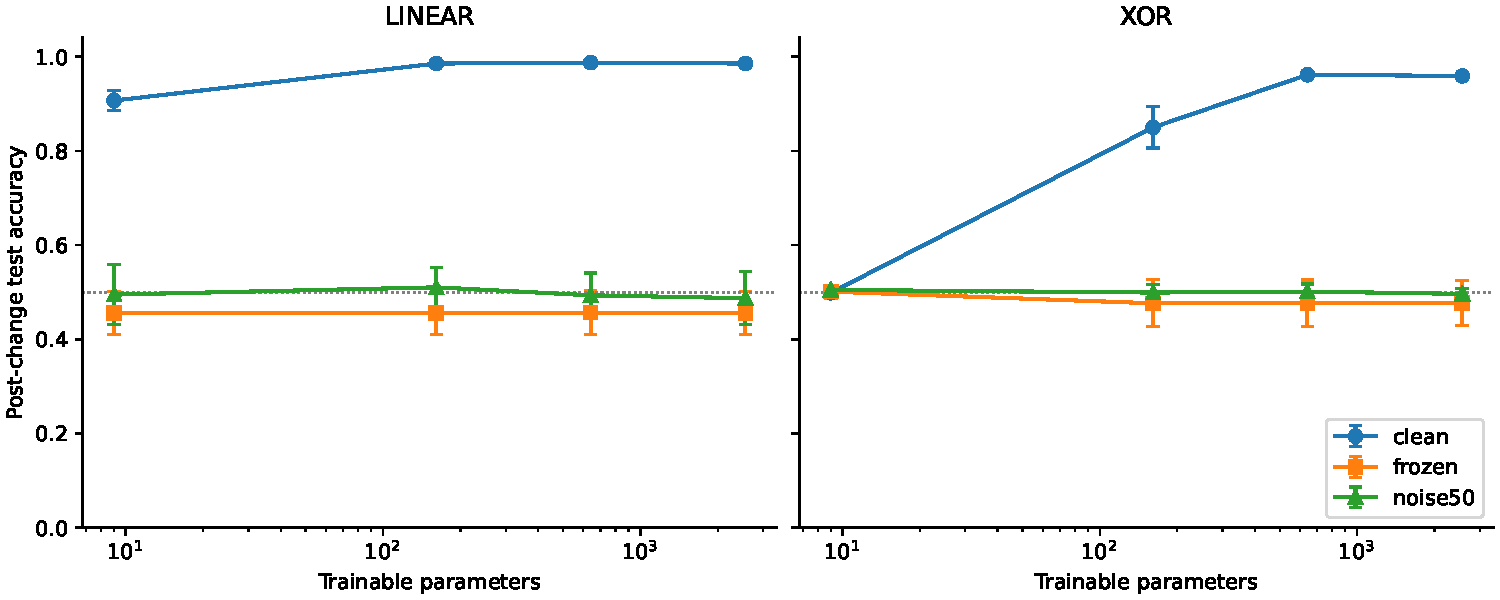
\includegraphics[width=\textwidth]{results/study-a-v2/capacity-feedback.pdf}
\caption{Capacity and feedback jointly determine observed accuracy. Error
bars are descriptive 95\% t intervals across 20 seeds. The dotted line is
chance accuracy; noisy feedback can coexist with information retained from
warmup, so individual noisy outcomes need not equal chance.}
\end{figure}

At an equal adaptation arithmetic proxy, the small model's 256 updates and
the largest model's 16 updates both cost 7,077,888 proxy FLOPs. The small
model leads by 42.80 points on linear tasks and 34.72 on XOR. However, it
receives sixteen times as many new examples, while the large model's warmup
cost is sixteen times greater. This is a particular compute/information trade,
not an isolated causal effect of feedback-loop efficiency or a scaling law.

\subsection{Feedback variations, transfer, and retention}
For the 161-parameter model, clean, 25\% corruption, and 50\% corruption yield
98.53\%, 92.05\%, and 51.03\% accuracy on linear tasks and 84.97\%, 71.84\%,
and 49.92\% on XOR. Inverted feedback yields 1.20\% and 13.32\% respectively.
More updates can reinforce the wrong target when the update rule assumes
trusted labels.

Delayed feedback reaches 98.28\% and 81.87\% at the online endpoint. After
flushing, its scores and final training losses equal clean feedback for every
seed and capacity. This equality is a correctness check for ordered updates,
not an additional empirical discovery about latency.

\begin{figure}[ht]
\centering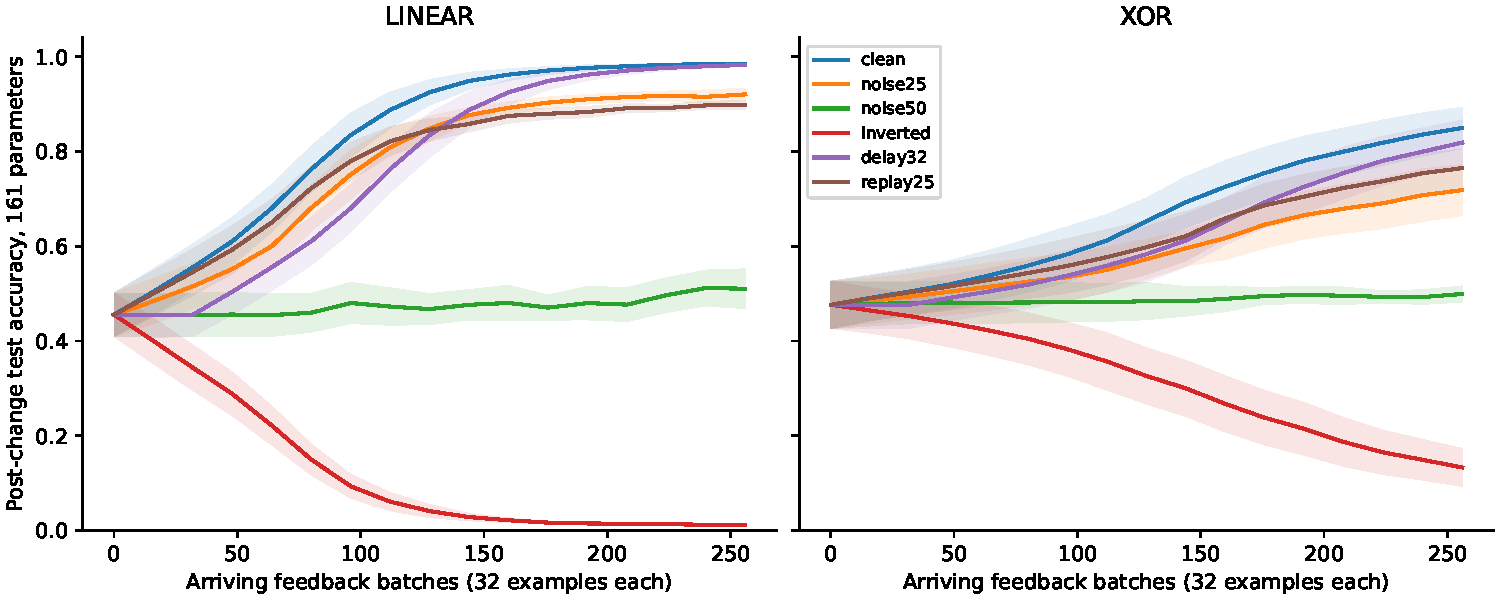
\includegraphics[width=\textwidth]{results/study-a-v2/learning-curves.pdf}
\caption{The same 161-parameter learner under six update conditions. Shading
shows descriptive 95\% seed-level intervals at fixed arrival checkpoints.}
\end{figure}

Clean small-model uniform-input accuracy is 98.44\% for linear rules and
88.19\% for XOR. This is distribution transfer within the same known rule
family, not transfer to an unrelated task. Old-rule accuracy after clean
adaptation is 45.23\% and 51.94\%. Replay raises these to 54.92\% and
64.43\% while lowering new-rule accuracy to 89.85\% and 76.48\%.
Because rules may conflict without a task identifier, this is an adaptation--
retention tradeoff; perfect performance on both is not always possible.

\subsection{Study B: feedback does not guarantee compositional gains}
\begin{table}[ht]
\centering
\caption{Study B mean constrained first-token accuracy (\%), 24 environments.
Direct tests use one command; composition tests use two. Chance is 12.5\%.}
\begin{tabular}{l r r r r r}
\toprule
Model & Direct none & Direct clean & Compose none & Compose clean & Compose oracle\\
\midrule
0.5B & 13.80 & 12.24 & 11.46 & 11.46 & 11.46\\
1.5B & 13.28 & 13.02 & 11.20 & 12.63 & 12.89\\
3B & 10.16 & 5.73 & 13.02 & 12.63 & 14.32\\
7B & 13.80 & 26.56 & 13.80 & 17.58 & 26.82\\
\bottomrule
\end{tabular}
\end{table}

For the primary 0.5B comparison, clean feedback and self-generated examples
both yield 11.46\% composition accuracy. The paired difference is 0.00 points
(95\% t CI [-1.03,1.03]; bootstrap [-0.78,1.04]). Clean-minus-none is also
0.00 points. This is a failure to demonstrate the hypothesized gain with this
mechanism, not proof that every feedback mechanism must fail.

The 7B model reaches 26.56\% on direct tasks with clean-16 examples versus
13.80\% without examples. Its composition scores are 17.58\% and 13.80\%,
respectively: a descriptive paired difference of 3.78 points (95\% CI
[0.38,7.17]). With explicit offsets, direct accuracy rises to 75.52\%, while
composition reaches 26.82\%. Representation of the instruction, inference of
the latent rule, and execution of compositions are distinct bottlenecks.

\begin{figure}[ht]
\centering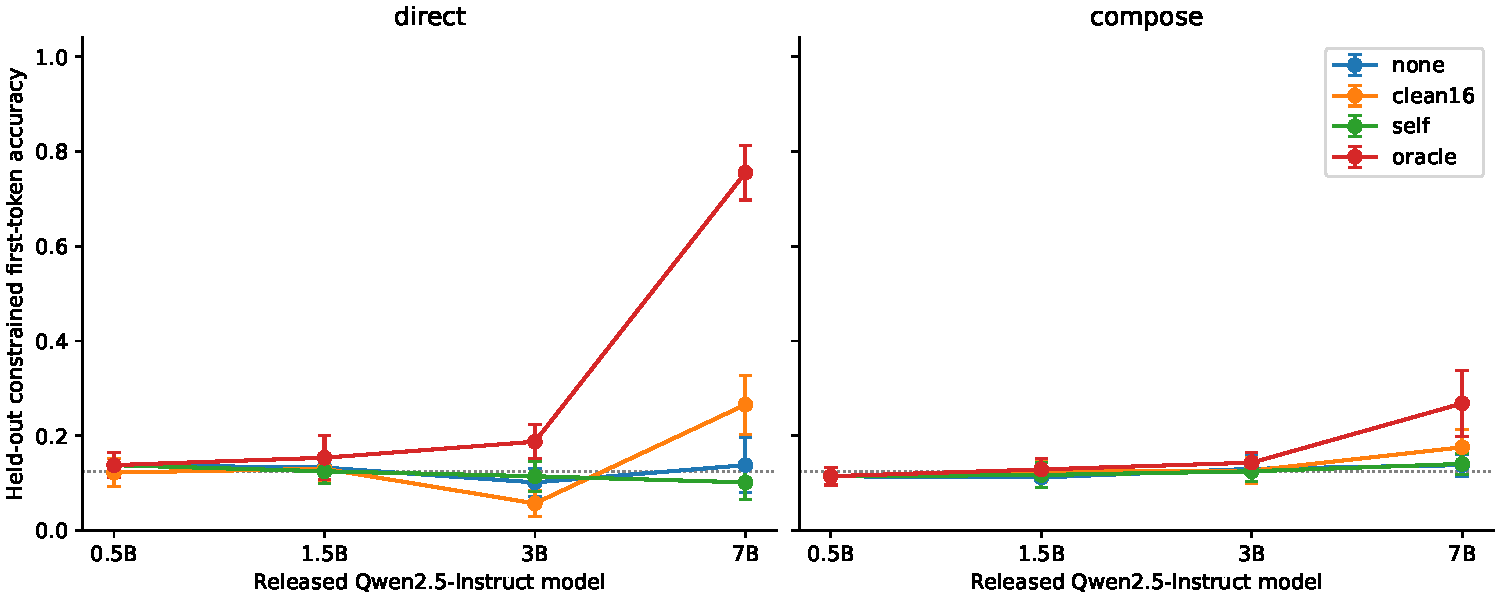
\includegraphics[width=\textwidth]{results/study-b-v1/language-model-feedback.pdf}
\caption{Released-model size and the supplied evidence affect direct and
compositional performance differently. Error bars are descriptive environment-
level 95\% t intervals. The oracle provides extra structured information;
it is not a cost-matched competitor.}
\end{figure}

LoRA trains 540,672 parameters in addition to the frozen 0.494B base. Without
example context, its direct accuracy is 26.30\% versus 13.80\% for the base.
The paired direct gain is 12.50 points (descriptive 95\% t CI [3.76,21.24]).
Composition accuracy is 13.15\%; its paired improvement over no-feedback base
is 1.69 points (95\% CI [-2.12,5.50]). Retaining examples at inference yields
13.28\% composition accuracy but reduces direct accuracy to 9.90\%.
Thus the persistent single-command gain is strongly context-dependent:
adding the same demonstrations does not preserve it. These results distinguish
a gain under the training prompt format from robust compositional transfer.

Each frozen-model suite processes 2,156,304 unpadded input tokens in 888
forward calls, including self-history construction and evaluation. Measured
suite times are 21.81, 56.22, 109.02, and 234.69 seconds; peak allocated memory
is 1.20, 3.41, 6.41, and 15.29 GiB. These figures are whole-suite accounting,
not equal lifetime budgets or per-condition causal estimates. The LoRA suite
adds 1,486,848 training input tokens and 86.67 measured update seconds. Its
extra optimization is explicitly not cost-matched to frozen inference.

\subsection{Limitations and interpretation}
Both studies use synthetic tasks with disclosed families and inexpensive
feedback. They do not measure autonomous exploration, long-horizon reward,
human intelligence, or general cross-domain skill accumulation. Study A's
fixed optimization schedule may interact with capacity. Its replay treatment
also changes fresh-example exposure. Study B uses only one model family and
a first-token response interface; low accuracy can reflect that interface,
insufficient prior execution ability, or the specific update schedule.

In development, 0.5B gave a surprising wrong response to a simple arithmetic
calibration. The official weight SHA-256 matched, and CPU float32, GPU
float32/bfloat16, and eager/SDPA paths reproduced it. These diagnostics exclude
some implementation failures but do not establish that the prompt or scoring
interface makes full use of model capability. A prospectively specified
full-generation follow-up is necessary before treating these negative results
as broadly representative of language agents.

The initial Study A random-stream defect and the corrected fresh-seed
replication are both disclosed and preserved. A disk-full error occurred only
during Study B export; every original run had completion metadata and complete
predictions. Export was repeated on a separate filesystem without rerunning
models. Source hashes and complete outcome grids were checked before analysis.

Prior work already establishes reinforcement learning, external memory,
verbal reflection, and test-time computation as relevant mechanisms. Our
current evidence is a diagnostic investigation of the stated hypothesis, not
a first discovery of feedback-driven intelligence. A targeted literature
review, especially its full-text coverage, remains incomplete.

\section{Conclusion}
Feedback enables substantial adaptation in small neural learners under task
change, but capacity remains consequential when both small and large models
learn. In our pretrained-language-model protocol, merely retaining correct
examples does not yield the hypothesized compositional improvement in the
smallest model. A short parameter-update schedule produces a persistent direct
skill gain without clear compositional transfer. These findings support
studying feedback quality, representation, and update mechanisms jointly.
They do not establish that feedback alone explains intelligence, or that
increasing model capacity is an incorrect research direction.

\begin{thebibliography}{11}
\bibitem{vaswani} A. Vaswani et al. Attention Is All You Need. NeurIPS, 2017.
\url{https://arxiv.org/abs/1706.03762}.
\bibitem{kaplan} J. Kaplan et al. Scaling Laws for Neural Language Models. 2020.
\url{https://arxiv.org/abs/2001.08361}.
\bibitem{hoffmann} J. Hoffmann et al. Training Compute-Optimal Large Language Models. 2022.
\url{https://arxiv.org/abs/2203.15556}.
\bibitem{chen} H. Chen et al. Feedback is all you need: from ChatGPT to autonomous driving. 2023.
\url{https://doi.org/10.1007/s11432-023-3740-x}. Bibliographic metadata verified;
full-text argument not assessed in this version.
\bibitem{duan} Y. Duan et al. RL$^2$: Fast Reinforcement Learning via Slow Reinforcement Learning. 2016.
\url{https://arxiv.org/abs/1611.02779}.
\bibitem{laskin} M. Laskin et al. In-context Reinforcement Learning with Algorithm Distillation. 2022.
\url{https://arxiv.org/abs/2210.14215}.
\bibitem{shinn} N. Shinn et al. Reflexion: Language Agents with Verbal Reinforcement Learning. 2023.
\url{https://arxiv.org/abs/2303.11366}.
\bibitem{madaan} A. Madaan et al. Self-Refine: Iterative Refinement with Self-Feedback. 2023.
\url{https://arxiv.org/abs/2303.17651}.
\bibitem{huang} J. Huang et al. Large Language Models Cannot Self-Correct Reasoning Yet. 2023.
\url{https://arxiv.org/abs/2310.01798}.
\bibitem{snell} C. Snell et al. Scaling LLM Test-Time Compute Optimally can be More Effective than Scaling Model Parameters. 2024.
\url{https://arxiv.org/abs/2408.03314}.
\end{thebibliography}
\end{document}
